\documentclass[tikz]{standalone}

\usepackage{tikz}
\usetikzlibrary{trees}
\usetikzlibrary{shapes}
\usetikzlibrary{positioning}
\usetikzlibrary{arrows.meta}

\tikzset{
    mynode/.style = {circle, ultra thick, draw=black, align=center,fill=yellow!30,font=\ttfamily\bfseries\Large,text=black},
    mynoder/.style = {circle, ultra thick, draw=black, align=center,fill=red!30,font=\ttfamily\bfseries\Large,text=black},
    mynodeb/.style = {circle, ultra thick, draw=black, align=center,fill=blue!30,font=\ttfamily\bfseries\Large,text=black},
    mynodeg/.style = {circle, ultra thick, draw=gray, align=center,fill=gray!05,font=\ttfamily\bfseries\Large,text=gray!20},
    mynodegr/.style = {circle, ultra thick, draw=gray, align=center,fill=gray!05,font=\ttfamily\bfseries\Large,text=red},
    edgen/.style = {-,ultra thick,black},
    edger/.style = {-,ultra thick,red},
    edgeb/.style = {-,ultra thick,blue},
    edgeg/.style = {-,ultra thick,gray},
    edgegd/.style = {-,ultra thick,brown,dashed}, % back
    edgevd/.style = {-,ultra thick,violet,dotted}, % forward
    edgexd/.style = {-,ultra thick,blue,densely dotted}, % traversal
    every picture/.style={/utils/exec={\ttfamily\bfseries}},
    every picture/.style={font issue=\ttfamily\bfseries},
    font issue/.style={execute at begin picture={#1\selectfont}}
}

\begin{document}

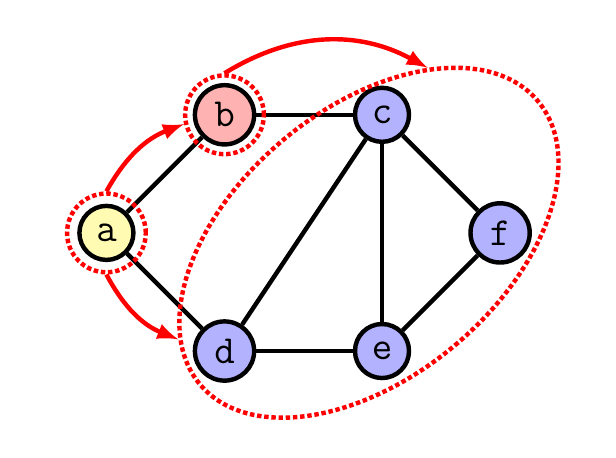
\begin{tikzpicture}[scale=1.00,transform shape]
%
\node[mynode] at (0.5,0) (a) {a};
\node[mynoder] at (2,1.5) (b) {b};
\node[mynodeb] at (4,1.5) (c) {c};
\node[mynodeb] at (2,-1.5) (d) {d};
\node[mynodeb] at (4,-1.5) (e) {e};
\node[mynodeb] at (5.5,0) (f) {f};
%
\draw[edgen] (a) edge node {} (b);
\draw[edgen] (a) edge node {} (d);
\draw[edgen] (b) edge node {} (c);
\draw[edgen] (c) edge node {} (e);
\draw[edgen] (e) edge node {} (d);
\draw[edgen] (f) edge node {} (c);
\draw[edgen] (e) edge node {} (f);
\draw[edgen] (d) edge node {} (c);

\node[ultra thick,draw=red,densely dotted,minimum size=1cm,circle] at (0.5,0) (C1) {};
\node[ultra thick,draw=red,densely dotted,minimum size=1cm,circle] at (2,1.5) (C2) {};
\node[ultra thick,draw=red,densely dotted,rotate around={-50:(3.8,-0.1)}, minimum width=3.4cm, minimum height=5.6cm,ellipse,anchor=center] at (2.4,-3) (C3) {};

\draw[edger,-latex] (C1.north) to[bend left=20] node {} (C2);
\draw[edger,-latex] (C1.south) to[bend right=20] node {} (C3);
\draw[edger,-latex] (C2.north) to[bend left=30] node {} (C3.north west);

\path[use as bounding box] (-0.5,-2.5) rectangle (6.5, 2.5);

\end{tikzpicture}

\newpage
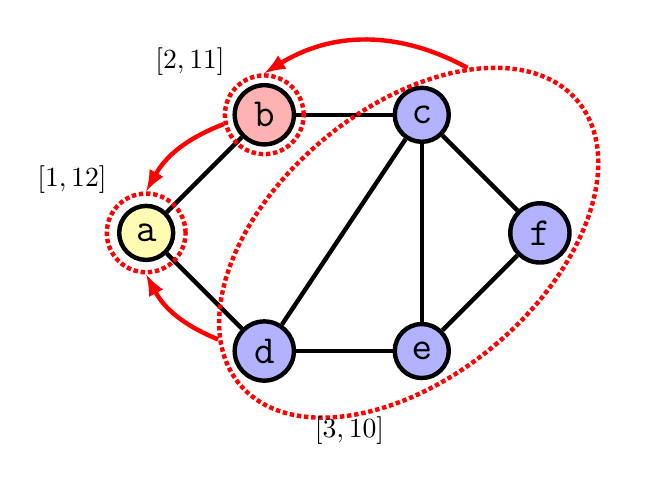
\begin{tikzpicture}[scale=1.00,transform shape]
%
\node[mynode] at (0.5,0) (a) {a};
\node[mynoder] at (2,1.5) (b) {b};
\node[mynodeb] at (4,1.5) (c) {c};
\node[mynodeb] at (2,-1.5) (d) {d};
\node[mynodeb] at (4,-1.5) (e) {e};
\node[mynodeb] at (5.5,0) (f) {f};
%
\draw[edgen] (a) edge node {} (b);
\draw[edgen] (a) edge node {} (d);
\draw[edgen] (b) edge node {} (c);
\draw[edgen] (c) edge node {} (e);
\draw[edgen] (e) edge node {} (d);
\draw[edgen] (f) edge node {} (c);
\draw[edgen] (e) edge node {} (f);
\draw[edgen] (d) edge node {} (c);

\node[ultra thick,draw=red,densely dotted,minimum size=1cm,circle,label={above left:$[1,12]$}] at (0.5,0) (C1) {};
\node[ultra thick,draw=red,densely dotted,minimum size=1cm,circle,label={above left:$[2,11]$}] at (2,1.5) (C2) {};
\node[ultra thick,draw=red,densely dotted,rotate around={-50:(3.8,-0.1)}, minimum width=3.4cm, minimum height=5.6cm,ellipse,anchor=center,label={below right:$[3,10]$}] at (2.4,-3) (C3) {};

\draw[edger,-latex] (C2) to[bend right=20] node {} (C1.north) ;
\draw[edger,-latex] (C3) to[bend left=20] node {} (C1.south);
\draw[edger,-latex] (C3.north west) to[bend right=30] node {} (C2.north);

\path[use as bounding box] (-0.5,-2.5) rectangle (6.5, 2.5);

\end{tikzpicture}

\newpage

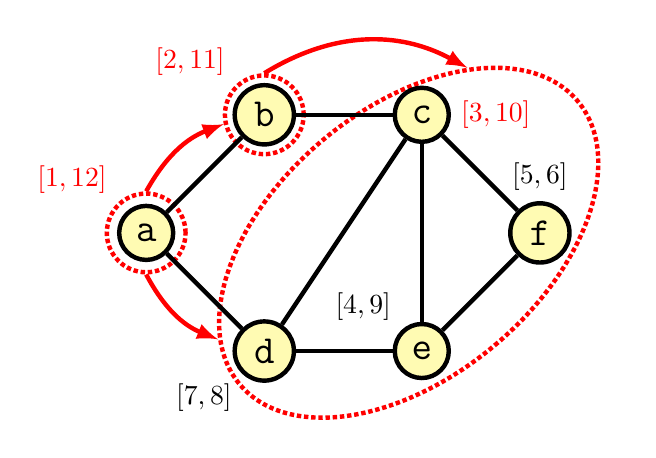
\begin{tikzpicture}[scale=1.00,transform shape]
\node[ultra thick,draw=red,densely dotted,minimum size=1cm,circle,label={[red]above left:$[1,12]$}] at (0.5,0) (C1) {};
\node[ultra thick,draw=red,densely dotted,minimum size=1cm,circle,label={[red]above left:$[2,11]$}] at (2,1.5) (C2) {};
\node[ultra thick,draw=red,densely dotted,rotate around={-50:(3.8,-0.1)}, minimum width=3.4cm, minimum height=5.6cm,ellipse,anchor=center] at (2.4,-3) (C3) {};

\draw[edger,-latex] (C1.north) to[bend left=20] node {} (C2) ;
\draw[edger,-latex] (C1.south) to[bend right=20] node {}  (C3);
\draw[edger,-latex] (C2.north) to[bend left=30] node {} (C3.north west);

%
\node[mynode] at (0.5,0) (a) {a};
\node[mynode] at (2,1.5) (b) {b};
\node[mynode, label={[red]right:$[3,10]$}] at (4,1.5) (c) {c};
\node[mynode, label={below left:$[7,8]$}] at (2,-1.5) (d) {d};
\node[mynode, label={above left:$[4,9]$}] at (4,-1.5) (e) {e};
\node[mynode, label={above:$[5,6]$}] at (5.5,0) (f) {f};
%
\draw[edgen] (a) edge node {} (b);
\draw[edgen] (a) edge node {} (d);
\draw[edgen] (b) edge node {} (c);
\draw[edgen] (c) edge node {} (e);
\draw[edgen] (e) edge node {} (d);
\draw[edgen] (f) edge node {} (c);
\draw[edgen] (e) edge node {} (f);
\draw[edgen] (d) edge node {} (c);


\path[use as bounding box] (-0.5,-2.5) rectangle (6.5, 2.5);


\end{tikzpicture}

\newpage

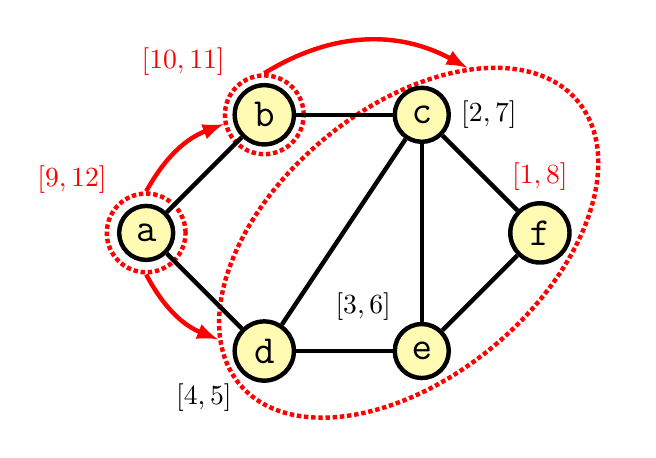
\begin{tikzpicture}[scale=1.00,transform shape]
\node[ultra thick,draw=red,densely dotted,minimum size=1cm,circle,label={[red]above left:$[9,12]$}] at (0.5,0) (C1) {};
\node[ultra thick,draw=red,densely dotted,minimum size=1cm,circle,label={[red]above left:$[10,11]$}] at (2,1.5) (C2) {};
\node[ultra thick,draw=red,densely dotted,rotate around={-50:(3.8,-0.1)}, minimum width=3.4cm, minimum height=5.6cm,ellipse,anchor=center] at (2.4,-3) (C3) {};

\draw[edger,-latex] (C1.north) to[bend left=20] node {} (C2) ;
\draw[edger,-latex] (C1.south) to[bend right=20] node {}  (C3);
\draw[edger,-latex] (C2.north) to[bend left=30] node {} (C3.north west);

%
\node[mynode] at (0.5,0) (a) {a};
\node[mynode] at (2,1.5) (b) {b};
\node[mynode, label={right:$[2,7]$}] at (4,1.5) (c) {c};
\node[mynode, label={below left:$[4,5]$}] at (2,-1.5) (d) {d};
\node[mynode, label={above left:$[3,6]$}] at (4,-1.5) (e) {e};
\node[mynode, label={[red]above:$[1,8]$}] at (5.5,0) (f) {f};
%
\draw[edgen] (a) edge node {} (b);
\draw[edgen] (a) edge node {} (d);
\draw[edgen] (b) edge node {} (c);
\draw[edgen] (c) edge node {} (e);
\draw[edgen] (e) edge node {} (d);
\draw[edgen] (f) edge node {} (c);
\draw[edgen] (e) edge node {} (f);
\draw[edgen] (d) edge node {} (c);


\path[use as bounding box] (-0.5,-2.5) rectangle (6.5, 2.5);

\end{tikzpicture}


\newpage

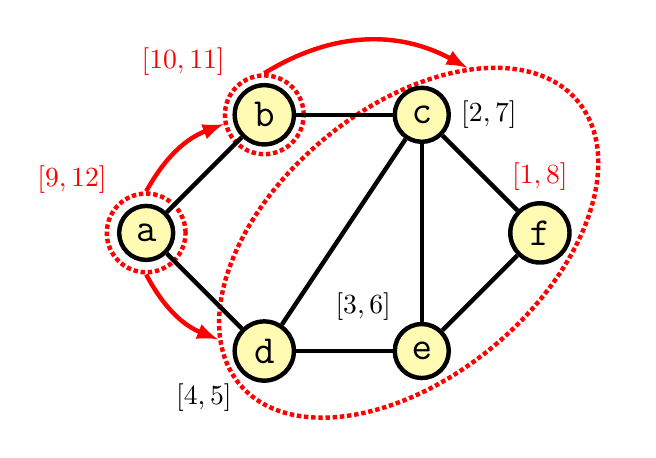
\begin{tikzpicture}[scale=1.00,transform shape]
\node[ultra thick,draw=red,densely dotted,minimum size=1cm,circle,label={[red]above left:$[9,12]$}] at (0.5,0) (C1) {};
\node[ultra thick,draw=red,densely dotted,minimum size=1cm,circle,label={[red]above left:$[10,11]$}] at (2,1.5) (C2) {};
\node[ultra thick,draw=red,densely dotted,rotate around={-50:(3.8,-0.1)}, minimum width=3.4cm, minimum height=5.6cm,ellipse,anchor=center] at (2.4,-3) (C3) {};

\draw[edger,-latex] (C1.north) to[bend left=20] node {} (C2) ;
\draw[edger,-latex] (C1.south) to[bend right=20] node {}  (C3);
\draw[edger,-latex] (C2.north) to[bend left=30] node {} (C3.north west);

%
\node[mynode] at (0.5,0) (a) {a};
\node[mynode] at (2,1.5) (b) {b};
\node[mynode, label={right:$[2,7]$}] at (4,1.5) (c) {c};
\node[mynode, label={below left:$[4,5]$}] at (2,-1.5) (d) {d};
\node[mynode, label={above left:$[3,6]$}] at (4,-1.5) (e) {e};
\node[mynode, label={[red]above:$[1,8]$}] at (5.5,0) (f) {f};
%
\draw[edgen] (b) edge node {} (a);
\draw[edgen] (d) edge node {} (a);
\draw[edgen] (c) edge node {} (b);
\draw[edgen] (e) edge node {} (c);
\draw[edgen] (d) edge node {} (e);
\draw[edgen] (c) edge node {} (f);
\draw[edgen] (f) edge node {} (e);
\draw[edgen] (c) edge node {} (d);


\path[use as bounding box] (-0.5,-2.5) rectangle (6.5, 2.5);

\end{tikzpicture}

\newpage
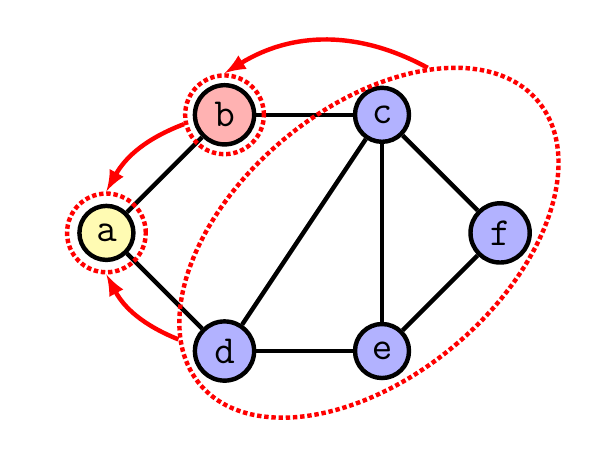
\begin{tikzpicture}[scale=1.00,transform shape]
%
\node[mynode] at (0.5,0) (a) {a};
\node[mynoder] at (2,1.5) (b) {b};
\node[mynodeb] at (4,1.5) (c) {c};
\node[mynodeb] at (2,-1.5) (d) {d};
\node[mynodeb] at (4,-1.5) (e) {e};
\node[mynodeb] at (5.5,0) (f) {f};
%
\draw[edgen] (b) edge node {} (a);
\draw[edgen] (d) edge node {} (a);
\draw[edgen] (c) edge node {} (b);
\draw[edgen] (e) edge node {} (c);
\draw[edgen] (d) edge node {} (e);
\draw[edgen] (c) edge node {} (f);
\draw[edgen] (f) edge node {} (e);
\draw[edgen] (c) edge node {} (d);

\node[ultra thick,draw=red,densely dotted,minimum size=1cm,circle] at (0.5,0) (C1) {};
\node[ultra thick,draw=red,densely dotted,minimum size=1cm,circle] at (2,1.5) (C2) {};
\node[ultra thick,draw=red,densely dotted,rotate around={-50:(3.8,-0.1)}, minimum width=3.4cm, minimum height=5.6cm,ellipse,anchor=center] at (2.4,-3) (C3) {};

\draw[edger,-latex] (C2) to[bend right=20] node {} (C1.north);
\draw[edger,-latex] (C3) to[bend left=20] node {} (C1.south);
\draw[edger,-latex] (C3.north west) to[bend right=30] node {} (C2.north);

\path[use as bounding box] (-0.5,-2.5) rectangle (6.5, 2.5);

\end{tikzpicture}


\end{document}